\section{Nähere Analyse der Implementierungsergebnisse}
\frame{\sectionpage}
\begin{frame}{Wiederholung}
\begin{itemize}
\item \textbf{Konservierung} \\
Eine LRP-Regel ist \textbf{konservativ} genau dann, wenn für die Relevanzwerte der Inputschicht und jeden Input $x$ gilt:
\begin{equation*}
\sum_i R_i(x) = f(x)
\end{equation*}
\item \textbf{Positivität} \\
Eine LRP-Regel ist \textbf{positiv} genau dann, wenn gilt:
\begin{equation*}
\forall x, i \quad R_i \geq 0
\end{equation*}
\item \textbf{Konsistenz} \\
Eine LRP-Regel ist \textbf{konsistent} genau dann, wenn sie \textbf{konservativ} und \textbf{positiv} ist.
\end{itemize}
\end{frame}

\begin{frame}{LRP-0}
\begin{equation*}
R_{j}=\sum_{k} \frac{a_{j} w_{j k}}{\sum_{i} a_{i} w_{i k}} R_{k}
\end{equation*}
\begin{itemize}
\item \textbf{konservativ:} \checkmark\footnote{Gilt hier und im Folgenden nur unter der Vorussetzung, dass der Bias nicht hinzuaddiert wird. Alle Bilder des Kapitels wurden unter Verwendung des Bias erstellt.}
\item \textbf{positiv:} \hspace{0.71cm} \textbf{X}
\item \textbf{konsistent:} \hspace{0.1cm} \textbf{X}
\end{itemize}
\includegraphics[width=\textwidth]{grafiken_theo/LRP-0_Check.png}
\end{frame}

\begin{frame}{LRP-$\epsilon$}
\begin{equation*}
R_{j}=\sum_{k} \frac{a_{j} w_{j k}}{\epsilon + \sum_{i} a_{i} w_{i k}} R_{k}
\end{equation*}
\begin{itemize}
\item \textbf{konservativ:} \textbf{X}
\item \textbf{positiv:} \hspace{0.71cm} \textbf{X}
\item \textbf{konsistent:} \hspace{0.1cm} \textbf{X}
\end{itemize}
\includegraphics[width=\textwidth]{grafiken_theo/LRP-eps_Check.png}
\end{frame}

\begin{frame}{LRP-$\epsilon$ - Abhängigkeit von $\epsilon$}
\begin{itemize}
\item Mit wachsendem $\epsilon$ verteilt sich die zurückgegebene Relevanz auf weniger Pixel
\item Das Rauschen der Relevanz nimmt ab und Konturen werden deutlicher
\end{itemize}
\includegraphics[width=0.95\textwidth]{grafiken_theo/Epsilon_Entwicklung.png}
\end{frame}

\begin{frame}{LRP-$\gamma$}
\begin{equation*}
R_{j}=\sum_{k} \frac{a_{j} \cdot \left(w_{j k} + \gamma \cdot w_{i j}^+ \right)}{\sum_{i} a_{i} \cdot \left(w_{j k} + \gamma \cdot w_{i j}^+ \right)} R_{k}
\end{equation*}
\begin{itemize}
\item \textbf{konservativ:} \checkmark
\item \textbf{positiv:} \hspace{0.71cm} \textbf{X}
\item \textbf{konsistent:} \hspace{0.1cm} \textbf{X}
\end{itemize}
\includegraphics[width=\textwidth]{grafiken_theo/LRP-Gamma_Check.png}
\end{frame}

\begin{frame}{LRP-$\gamma$ - Abhängigkeit von $\gamma$}
\begin{itemize}
\item Mit wachsendem $\gamma$ verlieren negative Relevanzen an Wert
\item Bildbereiche, die nicht zum klassifizierten Objekt gehören, werden "relevanter" \\
\item Es gilt LRP-$\gamma \xrightarrow {\gamma \rightarrow \infty} z^+$-Regel
\end{itemize}
\includegraphics[width=0.95\textwidth]{grafiken_theo/Gamma_Entwicklung.png}
\end{frame}

\begin{frame}{LRP-Komposition}
\begin{itemize}
\item Kombinierte Anwendung der vorherigen drei Regeln
\item Aus den Eigenschaften der einzelnen Regeln folgt, dass die Komposition weder positiv, noch konservativ ist.
\item Subjektiv betrachtet liefert diese Regel die interpretierbarsten Visualisierungen.
\vspace{1cm}
\end{itemize}
\includegraphics[width=\textwidth]{grafiken_theo/LRP-Comp_Check.png}
\end{frame}

\begin{frame}{$z^+$-Regel}
\begin{equation*}
R_{j}=\sum_{k} \frac{a_{j} \cdot w_{i j}^+}{\sum_{i} a_{i} \cdot w_{i j}^+} R_{k}
\end{equation*}
\begin{itemize}
\item \textbf{konservativ:} \checkmark
\item \textbf{positiv:} \hspace{0.71cm} \checkmark
\item \textbf{konsistent:} \hspace{0.1cm} \checkmark
\end{itemize}
\includegraphics[width=0.9\textwidth]{grafiken_theo/z+_Check.png}
\end{frame}

\begin{frame}{Übersicht Konservierung}
\begin{figure}
\includegraphics[width=0.85\textwidth]{grafiken_theo/relative_R_plots_374.png}
\end{figure}
\end{frame}


\section{Nähere Analyse der $z^+$-Regel}
\frame{\sectionpage}
\begin{frame}{Beobachtung}
\begin{itemize}
\item Die visualisierten Erklärungen für zwei verschiedene Klassen auf einem Bild ähneln sich sehr stark.
\item Bereits im drittletzten Dense-Layer wurde die Relevanz für beide Klassifikationen auf die gleichen Neuronen verteilt.
\end{itemize}
\includegraphics[width=\textwidth]{grafiken_theo/z+_vergleich.png}
\end{frame}

\begin{frame}{Vermutung}
\begin{itemize}
\item Negative Gewichte tragen stark zur Klassifizierung eines Objektes bei.
\item Durch das Ignorieren der Gewichte geht Information verloren.
\item Markante Features, die nicht oder negativ zur Klassifizierung beitragen, werden in der Backpropagation nicht gehemmt.
\end{itemize}
\begin{figure}
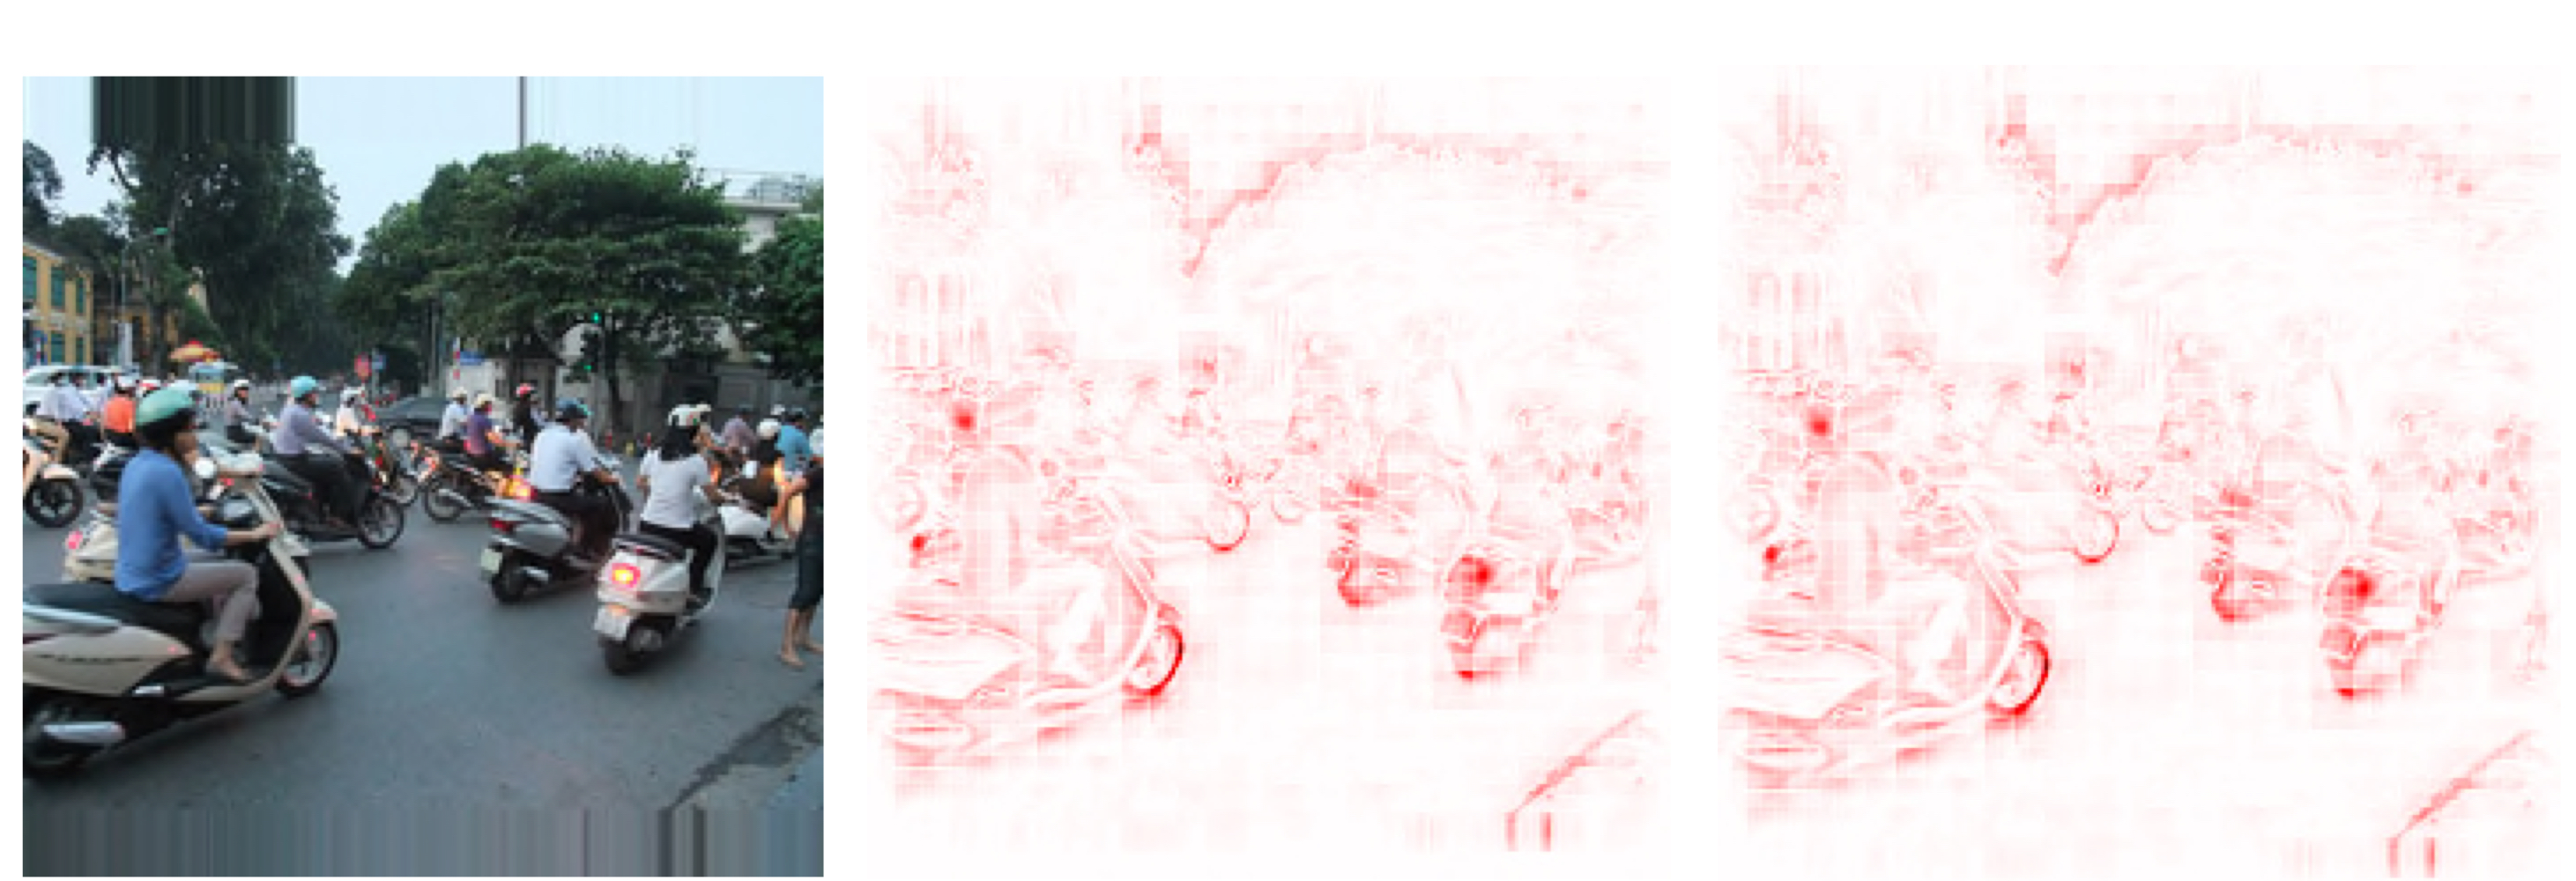
\includegraphics[width=0.65\textwidth]{grafiken_theo/expl_ai_z+.jpeg}
\caption{Implementierung der $z^+$-Regel durch Tool des Fraunhofer Instituts, angewendet auf Klassifizierung als \textit{Motorroller} und 
\textit{Motorradhelm}\footnote{https://lrpserver.hhi.fraunhofer.de/image-classification}.}
\end{figure}
\end{frame}